\documentclass{math}

\usepackage{enumerate}
\usepackage{graphicx}
\usepackage{tikz}

\geometry{letterpaper, margin=0.5in}

\title{Introduction to Intelligent Systems: Exam 1}
\author{Alvin Lin}
\date{August 2017 - December 2017}

\begin{document}

\maketitle

\subsection*{Problem 1: A* Search}
Trace the operation of  A* to the problem of getting from node \( F \) to node
\( G \) below using the heuristic of straight-line distance. Show the sequence
of nodes that the algorithms will consider and the \( f \), \( g \), and
\( h \) values for eachnode. Remove paths resulting in loops. When expanding
children, list the children in alphabetical order from left to right.
\[ h_{SLD}: \]
\begin{gather*}
  A = 15 \quad B = 10 \quad C = 12 \\
  D = 13 \quad F = 25 \quad P = 9 \\
  R = 10 \quad S = 8 \quad T = 22
\end{gather*}
\begin{center}
  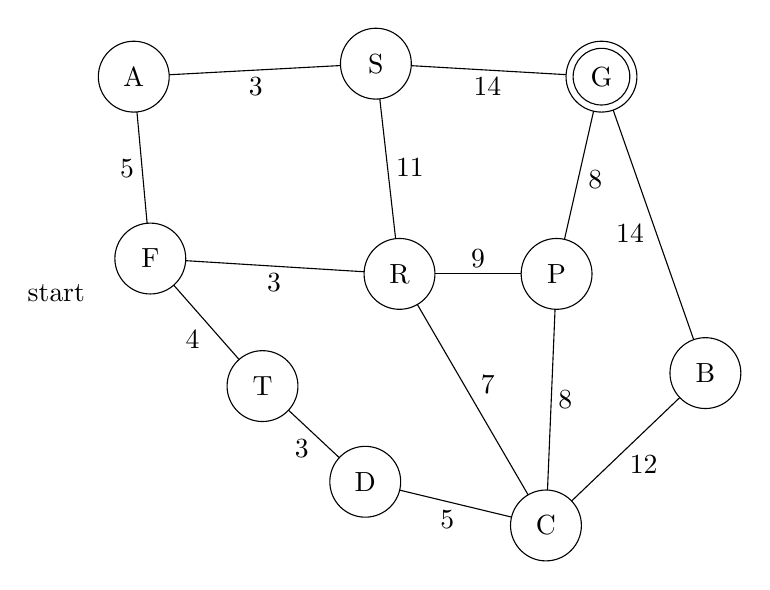
\begin{tikzpicture}[scale=0.15]
    \tikzstyle{every node}+=[inner sep=0pt]
    \draw [black] (36.6,-29.3) circle (3) node {R};
    \draw [black] (15.5,-28) circle (3) node {F};
    \draw [black] (49.9,-29.3) circle (3) node {P};
    \draw [black] (34.6,-11.5) circle (3) node {S};
    \draw [black] (33.7,-46.9) circle (3) node {D};
    \draw [black] (14.1,-12.6) circle (3) node {A};
    \draw [black] (25,-38.8) circle (3) node {T};
    \draw [black] (53.7,-12.6) circle (3) node {G};
    \draw [black] (53.7,-12.6) circle (2.4);
    \draw [black] (49,-50.6) circle (3) node {C};
    \draw [black] (62.5,-37.7) circle (3) node {B};
    \draw [black] (46.9,-29.3) -- (39.6,-29.3);
    \draw (43.25,-28.8) node [above] {9};
    \draw [black] (14.37,-15.59) -- (15.23,-25.01);
    \draw (14.17,-20.37) node [left] {5};
    \draw [black] (17.1,-12.44) -- (31.6,-11.66);
    \draw (24.44,-12.63) node [below] {3};
    \draw [black] (17.48,-30.25) -- (23.02,-36.55);
    \draw (19.71,-34.85) node [left] {4};
    \draw [black] (36.62,-47.61) -- (46.08,-49.89);
    \draw (40.65,-49.32) node [below] {5};
    \draw [black] (47.49,-48.01) -- (38.11,-31.89);
    \draw (43.45,-38.71) node [right] {7};
    \draw [black] (37.6,-11.67) -- (50.7,-12.43);
    \draw (44.05,-12.63) node [below] {14};
    \draw [black] (54.69,-15.43) -- (61.51,-34.87);
    \draw (57.34,-25.9) node [left] {14};
    \draw [black] (36.27,-26.32) -- (34.93,-14.48);
    \draw (36.26,-20.29) node [right] {11};
    \draw [black] (49.13,-47.6) -- (49.77,-32.3);
    \draw (50.01,-39.97) node [right] {8};
    \draw [black] (18.49,-28.18) -- (33.61,-29.12);
    \draw (25.97,-29.21) node [below] {3};
    \draw [black] (50.57,-26.37) -- (53.03,-15.53);
    \draw (52.55,-21.34) node [right] {8};
    \draw [black] (51.17,-48.53) -- (60.33,-39.77);
    \draw (57.27,-44.63) node [below] {12};
    \draw [black] (27.2,-40.84) -- (31.5,-44.86);
    \draw (28.33,-43.33) node [below] {3};
    \draw (10, -30.93) node [left] {start};
  \end{tikzpicture}
\end{center}
\begin{center}
  \begin{tabular}{|c|c|p{8cm}|c|}
    \hline
    Path & Current Node & Neighbors & Choice \\ \hline
    \( \emptyset \) & F &
      A: \( g(A) = 5; h(A) = 15; f(A) = 20 \) \newline
      R: \( g(R) = 3; h(R) = 10; f(R) = 13 \) \newline
      T: \( g(T) = 4; h(T) = 22; f(T) = 26 \)
      & R \\ \hline
    F & R &
      C: \( g(C) = 10; h(C) = 12; f(C) = 22 \) \newline
      S: \( g(S) = 14; h(S) = 8; f(S) = 22 \) \newline
      P: \( g(P) = 12; h(P) = 9; f(P) = 21 \)
      & P \\ \hline
    F,R & P &
      C: \( g(C) = 20; h(C) = 12; f(C) = 32 \) \newline
      G: \( g(G) = 20; h(G) = 0; f(G) = 20 \)
      & G \\ \hline
  \end{tabular} \\[0.5cm]
  Path: F,R,P,G
\end{center}

\subsection*{Problem 2: Minimax with alpha-beta pruning}
Fill in the following search tree assuming MAX goes first. Put an `X' over the
branch or tree that you can eliminate with alpha-beta pruning.
\begin{center}
  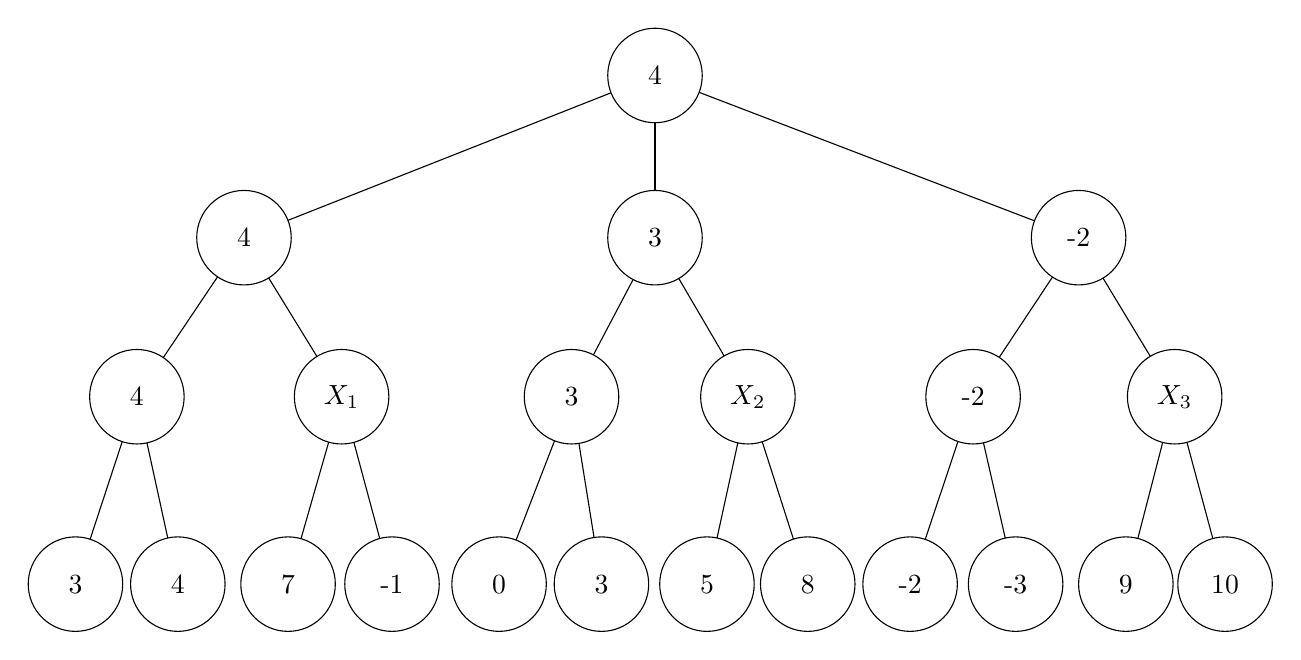
\begin{tikzpicture}[scale=0.2]
  \tikzstyle{every node}+=[inner sep=0pt]
  \draw [black] (40.2,-3.2) circle (3) node {4};
  \draw [black] (14.1,-13.5) circle (3) node {4};
  \draw [black] (40.2,-13.5) circle (3) node {3};
  \draw [black] (67.1,-13.5) circle (3) node {-2};
  \draw [black] (7.3,-23.6) circle (3) node{4};
  \draw [black] (20.3,-23.6) circle (3) node{\( X_1 \)};
  \draw [black] (34.9,-23.6) circle (3) node{3};
  \draw [black] (46.1,-23.6) circle (3) node{\( X_2 \)};
  \draw [black] (60.4,-23.6) circle (3) node{-2};
  \draw [black] (73.2,-23.6) circle (3) node{\( X_3 \)};
  \draw [black] (3.4,-35.5) circle (3) node {3};
  \draw [black] (9.9,-35.5) circle (3) node {4};
  \draw [black] (16.9,-35.5) circle (3) node {7};
  \draw [black] (23.5,-35.5) circle (3) node {-1};
  \draw [black] (30.3,-35.5) circle (3) node {0};
  \draw [black] (36.8,-35.5) circle (3) node {3};
  \draw [black] (43.5,-35.5) circle (3) node {5};
  \draw [black] (49.9,-35.5) circle (3) node {8};
  \draw [black] (56.4,-35.5) circle (3) node {-2};
  \draw [black] (63.1,-35.5) circle (3) node {-3};
  \draw [black] (70.1,-35.5) circle (3) node {9};
  \draw [black] (76.4,-35.5) circle (3) node {10};
  \draw [black] (37.41,-4.3) -- (16.89,-12.4);
  \draw [black] (40.2,-6.2) -- (40.2,-10.5);
  \draw [black] (43,-4.27) -- (64.3,-12.43);
  \draw [black] (12.42,-15.99) -- (8.98,-21.11);
  \draw [black] (15.67,-16.06) -- (18.73,-21.04);
  \draw [black] (38.81,-16.16) -- (36.29,-20.94);
  \draw [black] (41.71,-16.09) -- (44.59,-21.01);
  \draw [black] (6.37,-26.45) -- (4.33,-32.65);
  \draw [black] (7.94,-26.53) -- (9.26,-32.57);
  \draw [black] (19.48,-26.48) -- (17.72,-32.62);
  \draw [black] (21.08,-26.5) -- (22.72,-32.6);
  \draw [black] (33.82,-26.4) -- (31.38,-32.7);
  \draw [black] (35.37,-26.56) -- (36.33,-32.54);
  \draw [black] (45.46,-26.53) -- (44.14,-32.57);
  \draw [black] (47.01,-26.46) -- (48.99,-32.64);
  \draw [black] (65.44,-16) -- (62.06,-21.1);
  \draw [black] (68.65,-16.07) -- (71.65,-21.03);
  \draw [black] (59.44,-26.44) -- (57.36,-32.66);
  \draw [black] (61.06,-26.53) -- (62.44,-32.57);
  \draw [black] (72.44,-26.5) -- (70.86,-32.6);
  \draw [black] (73.98,-26.5) -- (75.62,-32.6);
  \end{tikzpicture}
\end{center}
The branch labeled \( X_1 \) can be pruned because a value of 7 was found in
the right branch, which is already greater than the max of 4 calculated in the
left branch. The branch labeled \( X_2 \) can be pruned because a value of 5
was found in the right branch, which is greater than the max of 3 calculated in
the left branch. The branch labeled \( X_3 \) can be pruned because a value of
9 was found in the right branch, which is greater than the max of -2 calculated
in the left branch.

\subsection*{Problem 3: Frogs and Toads}
Consider a two-player game featuring a board with four locations, numbered 1
through 4 and arranged in a line. Player A is a Toad and starts on space 1, and
player B is a Frog and starts on space 4, as shown in the diagram below. Player
A (Toad) moves first.
\begin{center}
  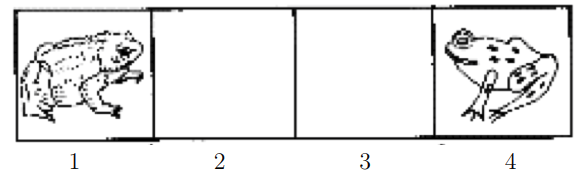
\includegraphics[width=12cm]{assets/frog_toad.png}
\end{center}
The two players take turns moving, and each player must move to an open
adjacent space in {\it either direction} (no wrap-around) as long as the move
is not off the board. If the opponent occupies an adjacent space, then the
player may jump over the opponent to the next open space if any. For example,
if Toad is on 3 and Frog is on 2, then Toad may move back to 1. \\[0.5cm]
The game ends when one player reaches the opposite end of the board.
If player Toad reaches space 4 first, then the value of the game is \( +1 \)
(a win for Toad); if player Frog reaches space 1 first, then the value of the
game is \( -1 \) (a win for Frog). \\[0.5cm]
Draw the complete game tree showing only legal moves. If a move results in a
loop (repeated state), then show the repeated state but do not expand it
further. Assume that Toad moves first and use the following conventions:
\begin{enumerate}
  \item Write each state as \( (s_{toad}, s_{frog}) \) where \( s_{toad} \) and
  \( s_{frog} \) denote the token locations. For example the start state is
  \( (1,4) \).
  \item Circle the terminal states (the leaves) and annotate each with its game
  value.
  \item Double-circle the loop states. Since it is not clear how to assign
  values to loop states, annotate each with a `?'.  Do not further expand a
  loop state.
  \item Mark each node with the backed-up minimax value.
\end{enumerate}
\begin{center}
  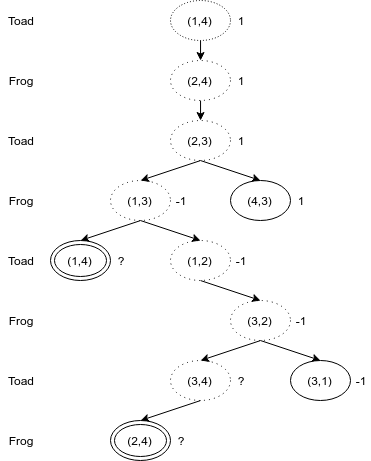
\includegraphics[width=12cm]{assets/frog_toad_diagram.png}
\end{center}

\begin{center}
  If you have any questions, comments, or concerns, please contact me at
  alvin@omgimanerd.tech
\end{center}

\end{document}
